\documentclass{article}
\usepackage[T1]{fontenc}
\usepackage{ae,aecompl}

% Ams math
\usepackage{amsmath}
\usepackage{amssymb}

% Figures
\usepackage{graphicx}

\usepackage{savetrees}

\graphicspath{img}

\newcommand{\tref}{t_{\textrm{ref}}}

\begin{document}
\title{Preliminary results on fitting to the AMOC data}
\author{Greg Ashton}
\date{}
\maketitle

In this document we show some preliminary results of fitting phenomological models
to the AMOC data. To select between these phenomological models we will use the
Bayes factor, defined as
\begin{align}
\mathcal{B} = \frac{P(\textrm{model A}| \textrm{ data})}{P(\textrm{model B}| \textrm{ data})}
\end{align}
such that $\mathcal{B} > 1$ provides evidence for model A over model B, while
$\mathcal{B} < 1$ provides evidence for model B over model A. 

We assume the data is a linear sum of the phenomological model and
gaussian noise to generate a likelihood function for the data. The Bayes factor
is sensitive to both how well the model fits the data, and also the priors chosen
for each model parameter. These priors have been chosen crudely from the data,
and so I will expect the Bayes factors to change when a more expert opinion is
applied.

To fit the models to the data, we have used MCMC simulations which estimate the
posterior distributions for each model parameters. To estimate the marginal
likelihood for each model $P(\textrm{model}| \textrm{ data})$ we have used
so-called `thermodynamic integration', this is a numerical method which has an
associated numerical error which we estimate.

In the following sections we will introduce each model starting with a basic
model, discuss the fit, and then compare between the models.

\section{Basic sinusoidal model}

\begin{align}
y(t) = y_0 + \dot{y}_0(t - \tref) + A_0 \sin\left(2\pi \frac{t}{P} + \psi_0\right)
\end{align}

\begin{figure}[htb]
\centering
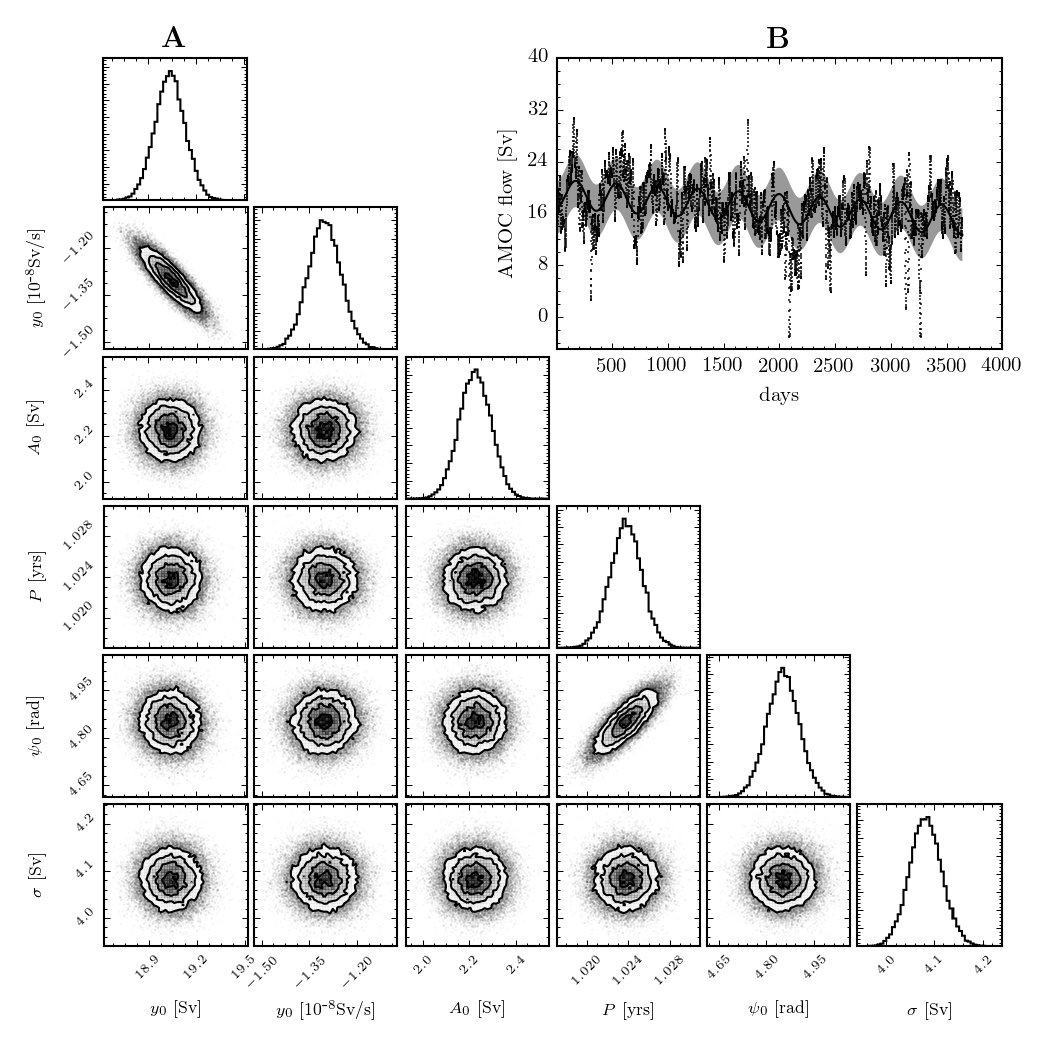
\includegraphics[width=0.8\textwidth]{img/BasicSinusoid_PosteriorWithFit}
\caption{}
\label{fig:}
\end{figure}

\section{Sinusoidal model with amplitude decay }

\begin{align}
y(t) = y_0 + \dot{y}_0(t - \tref) + (A_0 + \dot{A}_0(t-\tref)) \sin\left(2\pi \frac{t}{P} + \psi_0\right)
\end{align}

\begin{figure}[htb]
\centering
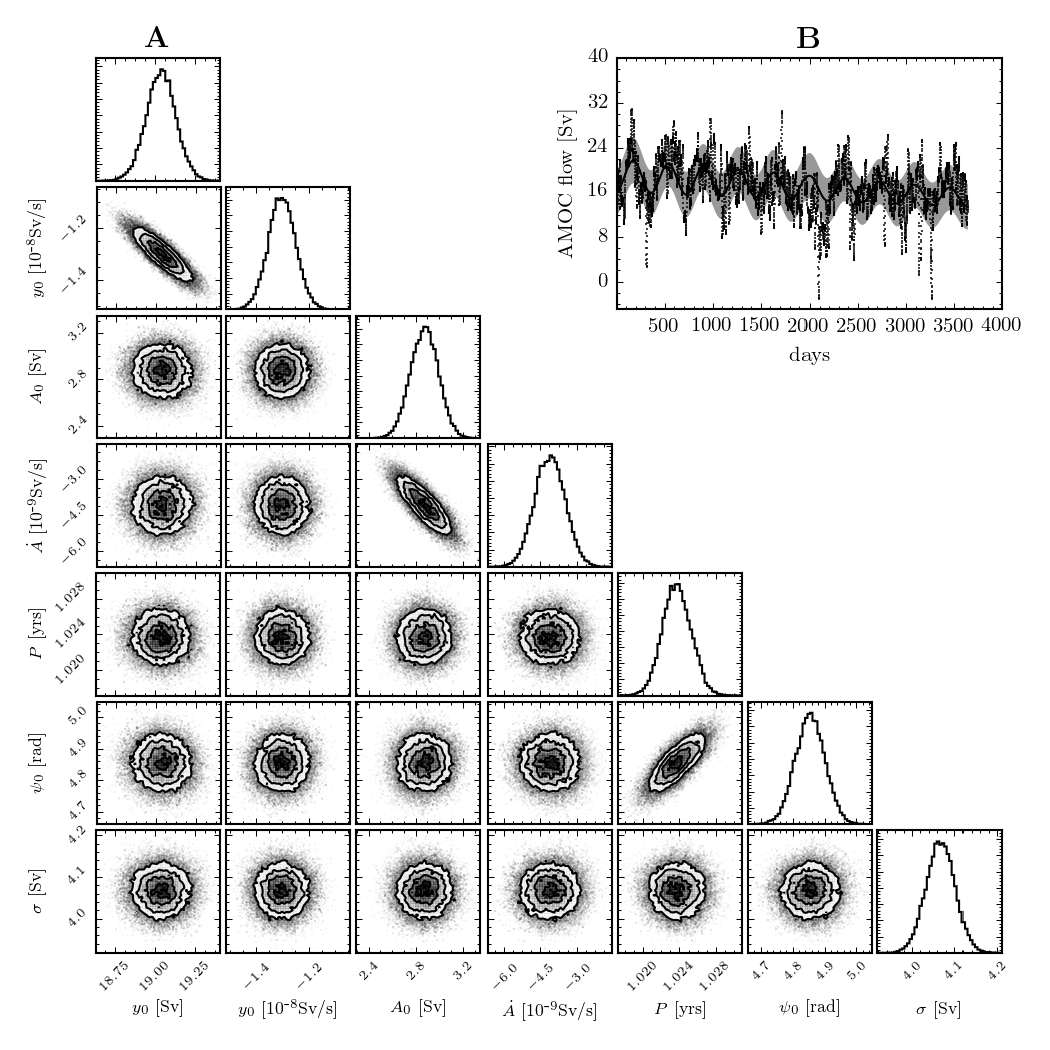
\includegraphics[width=0.8\textwidth]{img/BasicSinusoidAmplitudeDecay_PosteriorWithFit}
\caption{}
\label{fig:}
\end{figure}

\section{Sinusoidal model with amplitude decay and transient}

\begin{align}
y(t) = y_0 + \dot{y}_0(t - \tref) + (A_0 + \dot{A}_0(t-\tref)) \sin\left(2\pi \frac{t}{P} + \psi_0\right)
\end{align}

\begin{figure}[htb]
\centering
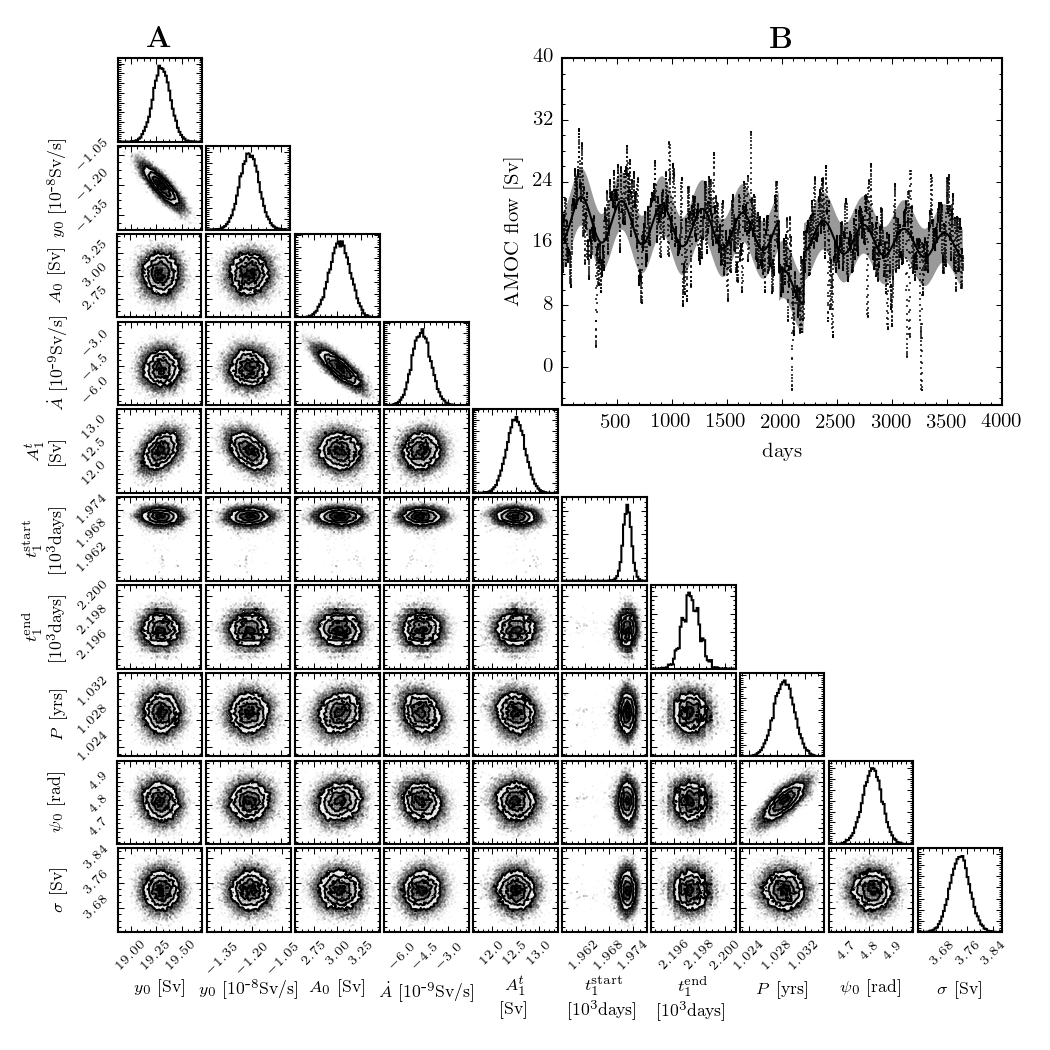
\includegraphics[width=0.8\textwidth]{img/BasicSinusoidAmplitudeDecayWithTransient_PosteriorWithFit}
\caption{}
\label{fig:}
\end{figure}






\end{document}
